
\begin{enumerate}
    \item A beaker of radius \(r\) is filled with water (refractive index \(\frac{4}{3}\)) up to a height \(H\) as shown in the figure on the left. The beaker is kept on a horizontal table rotating with angular speed \(\omega\). This makes the water surface curved so that the difference in the height of water level at the center and at the circumference of the beaker is \(h\) (\(h \ll H\), \(h \ll r\)), as shown in the figure on the right. Take this surface to be approximately spherical with a radius of curvature \(R\). Which of the following is/are correct? (\(g\) is the acceleration due to gravity)
        \begin{tasks}(2)
            \task \(R = \frac{h^2 + r^2}{2h}\)
            \task \(R = \frac{3r^2}{2h}\)
            \task Apparent depth of the bottom of the beaker is close to \(\frac{3H}{2} \left(1 + \frac{\omega^2H}{2g}\right)^{-1}\)
            \task Apparent depth of the bottom of the beaker is close to \(\frac{3H}{4} \left(1 + \frac{\omega^2H}{4g}\right)^{-1}\)
        \end{tasks}
\end{enumerate}
\begin{center}
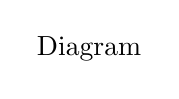
\begin{tikzpicture}
    \node {Diagram};
\end{tikzpicture}
\end{center}
